\documentclass[tocnosub,noragright,centerchapter,12pt,fullpage]{uiucecethesis09}


% Use draftthesis for notes and date markings on every page.  Useful when you
%   have multiple copies floating around.
% Use offcenter for the extra .5 inch on the left side. Needed with fullpage and fancy.
% Use mixcasechap for compatibility with hyperref package, which does NOT like all caps default
% Use edeposit for the adviser/committee on the title page.
% Use tocnosub to suppress subsection and lower entries in the TOC.
% PhD candidates use "proquest" for the proquest abstract.

\makeatletter

%%%%%%%%%%%%%%%
% MK Added to make bib work
% \bstctlcite{IEEEexample:BSTcontrol}

% MK added to highlight stuff
\usepackage{color,soul}

% MK added so figures can use the [H] option and be put where I want them.
\usepackage{float}

% MK added so algorithms work
\usepackage{algorithm}

%%%%%%%%%%%%%%%

\setcounter{secnumdepth}{5} % to make subsubsections work
\usepackage{setspace}
\usepackage{epsfig}  % for figures
\usepackage{graphicx}  % another package that works for figures
\usepackage{subfigure}  % for subfigures
\usepackage{amsmath}  % for math spacing
\usepackage{amssymb}  % for math spacing
%\usepackage{url}  % Hyphenation of URLs.
\usepackage{lscape}  % Useful for wide tables or figures.
\usepackage[justification=raggedright]{caption}	% makes captions ragged right - thanks to Bryce Lobdell

\DeclareMathOperator*{\argminA}{arg\,min} % Jan Hlavacek

% Uncomment the appropriate one of the following four lines:
%\phdthesis
%\phdthesis
%\otherdoctorate[abbrev]{Title of Degree}
%\othermasters[abbrev]{Title of Degree}

\title{Automated Isotope Identification Using Artificial Neural Networks}
\author{Mark Kamuda}
\department{Nuclear Plasma and Radiological Engineering}
%\department{\mbox{Nuclear, Plasma, and Radiological Engineering}}
\degreeyear{2018}

% Advisor name is required for
% - doctoral students for the ProQuest abstract
% - master's students who do not have a master's committee
% \advisor{Assistant Professor Clair J. Sullivan}

% Uncomment the \committee command for
% - all doctoral students
% - master's students who have a master's committee
\committee{Professor Kathryn Huff, Adviser\\
        Professor Rizwan Uddin\\
        Professor Tomasz Kozlowski\\
        Professor Clair Sullivan\\
        Professor Mark Hasagawa-Johnson}





\begin{document}

%%%%%%%%%%%%%%%%%%%%%%%%%%%%%%%%%%%%%%%%%%%%%%%%%%%%%%%%%%%%%%%%%%%%%%%%%%%%%%%
% COPYRIGHT
%
%\copyrightpage
%\blankpage

%%%%%%%%%%%%%%%%%%%%%%%%%%%%%%%%%%%%%%%%%%%%%%%%%%%%%%%%%%%%%%%%%%%%%%%%%%%%%%%
% TITLE
%
\maketitle

%\raggedright
\parindent 1em%

\frontmatter


\begin{abstract}


There is a need to develop an algorithm that can identify and quantify isotopes in low-resolution gamma-ray spectra. Trained gamma-ray spectroscopists typically rely on intuition when identifying isotopes in spectra. Because they incorporate something similar to intuition, pattern recognition algorithms such as neural networks are prime candidates for automated isotope identification. Algorithms based on feature extraction such as peak finding or ROI algorithms work well for well-calibrated high resolution detectors. For low-resolution detectors, it may be more beneficial to use algorithms that incorporate more abstract features of the spectrum. To solve this, an artificial neural network (ANN) was trained to predict the presence and relative activities of isotopes from a mixture of many isotopes. The ANN is trained with simulated gamma-ray spectra, allowing easy expansion of the library of target isotopes. This proposal outlines extensions to this work including investigating new datasets and ANN structures.

\end{abstract}

\tableofcontents

\listoftables

\listoffigures

\mainmatter


\chapter{Introduction}

The main question addressed in this work is: Can artificial neural networks (ANNs) using simulated spectra as training data automate isotope identification and quantification? Gamma-ray spectroscopists often use intuition when identifying isotopes in spectra. ANNs mimic this abstract analysis, synthesizing features of a gamma-ray spectrum in non-intuitive ways. Exploiting this intuition may overcome common hurdles encountered by other isotope identification algorithms. 

% This may give ANNs the ability to identify and quantify isotopes using large isotope libraries practical for domestic nuclear security, operate using low-resolution NaI radiation detectors without knowing the detector calibration or background spectrum.

% The idea to use ANNs first came as a method to exploit a potential data source in post-detonation nuclear forensics. After the device explodes, first responders will likely flood the affected area. Some of these responders will be fitted with gamma-ray spectrometers, the cheapest and most common being some size of NaI(Tl) scintillation crystals. While these crystals produce a gamma-ray spectrum with somewhat poor resolution, their potential ubiquity over heavier, more expensive systems that may require a day to cool (HPGe need liquid nitrogen temperatures to operate. This requires mechanical cooling or a dewar of liquid nitrogen. Regardless of the cooling method, they require about a day to cool if not already at operational temperature.) make them a potential source of a mountain of spectroscopic data from blast debris. This spectroscopic data can be used to identify the isotopes and their ratios in the debris. This data can be used to begin the process of attribution. Currently, the isotopics are calculated by sending debris samples to a few labs around the country (one of which is the Counting Room in the C-NR division at LANL). The debris is then chemically separated into constituent fission products, and those fission products are counted using well shielded HPGe detectors to very accurately determine isotopics. While this process will result in a more accurate measure of debris isotopics, the time necessary to transport, perform the chemical separation for each piece of debris, and measure the debris with the HPGe detectors may be on the order of days. While this may sound quick, this time will sacrifice some of the short-lived isotopes in the debris. In addition to this, if attribution time can be shortened from days to hours, international response could be organized quicker. 

% Current gamma-ray spectroscopy techniques may be inadequate to be used for post-detonation debris analysis. Feature extraction techniques typically rely on fitting non-overlapping gamma-ray peaks. In post-detonation debris, many isotopes will be emitting gamma-rays, creating multiple overlapping gamma-lines. Template matching algorithms may need an excessively large library to handle this task. Each sample of debris will contain tens of isotopes in complicated combinations. These exact combinations may be hard to determine  \textit{a priori} due to differences in device design and fractionation effects. 



The proposed work will demonstrate the performance of ANNs for automated gamma-ray spectroscopy in low-resolution spectra. The low-resolution detector of interest in this work is a 2-inch by 2-inch NaI(Tl) cylindrical scintillation detector. This detector is industry standard due to its ease of use, low cost, and acceptable resolution for gamma-ray spectroscopy. 

The performance of each algorithm will be displayed on two different datasets. The first dataset will focus on identifying isotopes in ANSI N42-34-2006, the American national standard performance criteria for hand-held instruments for the detection and identification of radionuclides \cite{ANSI}. The second dataset will be built to perform uranium enrichment calculations.

% This may give ANNs the ability to identify and quantify isotopes using large isotope libraries practical for domestic nuclear security, operate using low-resolution NaI radiation detectors without knowing the detector calibration or background spectrum.

% Tasks investigated here will focus on identifying isotopes in the ANSI N42-34-2006 required list \cite{ANSI}. This ANSI standard also requires isotope identification algorithms to operate when the radioactive material is behind shielding. Accordingly, the impact of shielding will also be incorporated into this work. 

In addition to isotope identification, this work will explore the ability of ANNs to quantify the count contribution from each isotope. The ANN's ability to extract count contribution information from gamma-ray spectra is important for nondestructive analysis (NDA), such as uranium enrichment calculations. Knowing the enrichment of uranium is important in two scenarios. The first scenario is when uranium is identified at a border crossing. Typically the spectrum would need to be given to a trained spectroscopist to quantify the enrichment, but this process could be automated on the device first used to identify it. The second case would be in treaty verification technologies. Low-resolution NaI gamma-ray detectors decrease the amount of possibly sensitive information while giving enough information to produce accurate enrichment quantification. The fact that ANNs can be taught to ignore certain patterns and only give information agreed upon by treaty signatories also makes them a good tool for treaty verification. The ability of ANNs to operate without knowing the shielding and background spectrum makes them better for zero knowledge scenarios. NaI detectors also have a higher efficiency than the higher resolution HPGe. This means that the counting times for NaI are smaller than would be required to get the same number of counts using an HPGe.    

% The second purpose is a possible use of neural networks in post-detonation nuclear forensics. In post-detonation nuclear forensics, a large number of radioactive fission products are created. Quantifying the amount of isotopes in post-detonation debris can yield useful information about the device's properties. Mixtures of laboratory sources will be used as a surrogate for post-detonation debris and the ability for the ANN to accurately calculate the mixture components will be established.

% Another case where knowing the isotope 





% An ANN will learn to perform these tasks by learning from simulated datasets that represent these tasks. The aim of this work is to demonstrate that an ANN can be taught to perform different isotope identification tasks using a simulated dataset using the same general training method.









\chapter{Literature Review}


\section{Gamma-Ray Spectroscopy for Isotope Identification}

Traditionally, isotope identification is conducted by a trained spectroscopist. Rawool-Sullivan et al. identified a common workflow performed by a group of gamma-ray spectroscopists \cite{Sullivan2010}. This workflow includes discriminating background and source photopeaks, adjusting the calibration using background photopeaks and checking for shielding effects in the low-energy photopeaks. Once photopeaks are identified, the spectroscopist would use their prior knowledge of isotope emissions (or consult a database of these emissions) to match isotopes to the spectrum. The researchers also noted that while  spectroscopists used this book knowledge, they often would use intuition developed from analyzing tens or hundreds of gamma-ray spectrum. The researchers also noted the difficulty in incorporating this subjective analysis into an automated algorithm.
% This is one of the main arguments for using ANNs in automated isotope ID


There are many automated radioisotope identification methods available, but few perform well given a low-resolution gamma-ray spectrum of a mixture of radioisotopes. Common methods include library comparison algorithms, region of interest (ROI) algorithms, principle component analysis (PCA), and template matching.

Library comparison algorithms attempt to match photopeak energies found in a gamma-ray spectrum with those found in a library of known isotope decay energies. Drifts and uncertainties in detector calibration can lead to misidentifying photopeaks, leading to incorrect isotope identifications \cite{burr2009}. To be automated, this method needs an algorithm to extract photopeak centroids despite calibration drift and unknown background radiation. Photopeak extraction algorithms face difficulties when a large number of photopeaks overlap in a spectrum, such as when a mixture of radio-isotopes are measured with a low-resolution detector \cite{xiong2015}.

ROI algorithms search for elevated counts compared to background in a region where target radioisotope photopeaks are expected. ROI algorithms may also operate poorly when photopeaks of different radioisotopes overlap \cite{burr2009}. For this reason, large isotope libraries will perform poorly using this method. Similarly to the library comparison algorithm, calibration drift may shift photopeaks into different neighboring ROIs, leading to incorrect identification. The ROI method has been used to differentiate normally occurring radioactive material (NORM) from special nuclear material (SNM) using plastic scintillators \cite{Ely2006}.

PCA can also be applied to radioisotope identification. The goal of PCA is to reduce the dimensionality of a dataset into uncorrelated variables \cite{Jolliffe2002}. Using a few of these principle components, the data may be represented in a reduced space that contains most of the information present in the original data. The transformed data can then be clustered based on isotope identity. Clustering algorithms may include K-means or Mahalanobis distance \cite{Kanungo2002, Kumari2012}. PCA has been applied to isotope identification using plastic scintillators \cite{Boardman2012} and anomaly detection using both plastic scintillators and NaI detectors \cite{runkle2006b}. Despite the progress of PCA in some isotope identification problems, there has not been significant progress in applying PCA to separating mixtures of isotopes in gamma-ray spectra.

Template matching algorithms find an example in a database of gamma-ray spectra that most closely matches a measured spectrum \cite{burr2009}. The database of spectra can contain multiple detector calibration settings, shielding materials, and source-to-detector distances. Goodness of fit can be measured using a hypothesis test such as chi-squared test, euclidean distance, or Mahalanobis distance. While a sufficient amount of example spectra can be used to identify almost any measured spectrum, the drawback of this method is the time necessary to compare a measured spectrum to the library and the computer memory necessary to store said library. This method also may have difficulty when mixtures of isotopes are considered, although work is being done to correct this \cite{mattingly2010}.

These algorithms largely incorporate book knowledge. By further incorporating the intuition identified by Rawool-Sullivan et al., these algorithms may be improved. A machine learning approach to automated gamma-ray spectroscopy may be able to marry book knowledge and a trained spectroscopists intuition.  




\section{Artificial Neural Networks}

Artificial neural networks were first created to mimic biologic neurons. Since their creation, they have demonstrated promising results on a variety of different classification and regression tasks \cite{Jeyanthia2015, Krizhevsky2012, Rababaah2015}. The following sections will give an overview of how ANNs learn and operate.


\subsection{Architecture and Training}

ANNs work by mapping an arbitrary input vector, $\mathbb{R}^N$, to an arbitrary output vector, $\mathbb{R}^K$, where $N$ and $K$ are positive integers. An example ANN that maps $\mathbb{R}^N$ $\mapsto$ $\mathbb{R}^K$ is shown in Figure \ref{fig:Network}. In this figure, each circle represents a neuron, also called a node. The $A_{n}$ nodes are the input and the $C_{k}$ nodes are the output. The $B_{j}$ nodes are the hidden layer. Adding additional hidden layers and nodes in each layer increases the degrees of freedom available to the ANN. Additional degrees of freedom let the ANN represent more complicated functions. The lines connecting nodes in the ANN are weight coefficients that propagate information from one layer to another. 


The mathematical process governing each neuron in the ANN is shown in Figure \ref{fig:Node}. In Figure \ref{fig:Node}, the signal from the previous layer is propagated to the next by applying some function to the dot product of the signal from the previous layer and the weight vector going into a given node, B$_{j}$ in Figure \ref{fig:Node}. The activation function is typically a monotonic `S'-shaped curve, such as any sigmoidal function. Given a one-layer ANN with a finite number of hidden nodes, any function $\mathbb{R}^N$ $\mapsto$ $\mathbb{R}^K$ can be described to arbitrary precision \cite{hornik1991}. There is no direct method to compute the optimal number of hidden layers or nodes for a given problem. The number of hidden layers and nodes per layer, along with other hyperparameters, need to be optimized for a given dataset.

\begin{figure}[H]
    \centering
    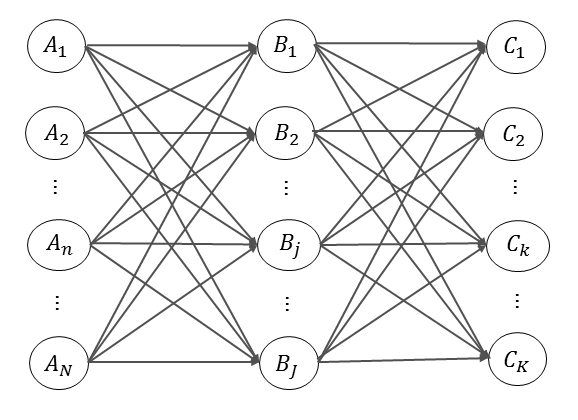
\includegraphics[width=0.5\linewidth]{images/Network}
    \caption{Example ANN with input layer A, hidden layer B, and output layer C.}
    \label{fig:Network}
\end{figure}

\begin{figure}[H]
	\centering
	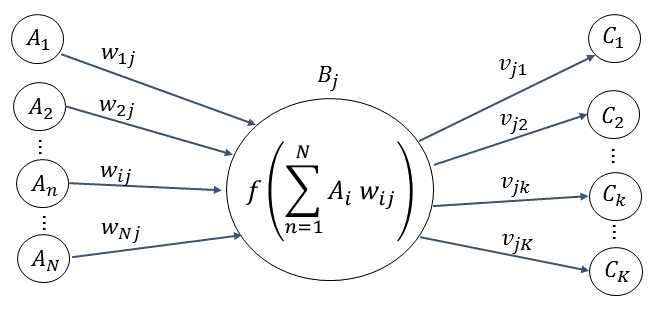
\includegraphics[width=0.55\linewidth]{images/Node_ABC_2}
	\caption{Summary of the operation of a single neuron.}
	\label{fig:Node}
\end{figure}

Artificial ANNs learn a function by changing the weights connecting the layers so that some error function is minimized for a given dataset. One popular method to update the weights is through the process of gradient descent through the backpropogation of errors \cite{Rumelhart1986}. The corresponding update equation for a single weight, $w_j$, can be computed as 

\begin{equation} \label{eq:update1}
\Delta w_{j} = - \eta \frac{dE(\boldsymbol{y}(\boldsymbol{x}),\hat{\boldsymbol{y}}(\boldsymbol{x}))}{dw_j}
\end{equation}

and 

\begin{equation} \label{eq:update2}
w^{new}_{j} = w^{old}_{j} + \Delta w_{j}.
\end{equation}

In Equations \ref{eq:update1} and \ref{eq:update2}, $E$ is the given error function to be minimized (commonly mean squared error or cross entropy) and $\eta$ is the learning rate of the ANN. For a given set of input data, $\boldsymbol{x}$, the error function compares the ground truth, $\boldsymbol{y}(\boldsymbol{x})$, with the models output, $\hat{\boldsymbol{y}}(\boldsymbol{x})$. During the weight update process, the available data is split into two sets, a training and a validation set. The training data is used to update the weights using Equation \ref{eq:update2}. Using a process called early stopping, the training is continued until the error on the validation dataset, $E(\boldsymbol{y}(\boldsymbol{x}_{validation}),\hat{\boldsymbol{y}}(\boldsymbol{x}_{validation}))$, stops decreasing. An example of easily stopping is illustrated in Figure \ref{fig:training_validation_error}. Without early stopping, the error on the validation set may start increasing, despite the error on the training set decreasing. This indicates that the ANN is memorizing the training set and failing to generalize to data outside the training set.


\begin{figure}[H]
    \centering
    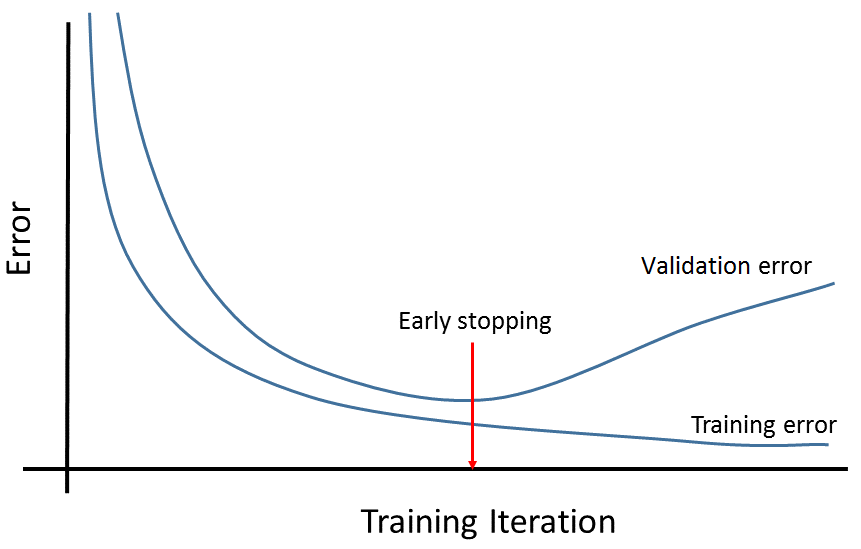
\includegraphics[width=0.6\linewidth]{images/training_validation_error}
    \caption{Ideal training and validation error curves.}
    \label{fig:training_validation_error}
\end{figure}



\subsection{Hyperparameters}

In general, ANNs have a tendency to memorize their training set in a process called overtraining. An overtrained ANN will tend to incorrectly identify novel data. To prevent this, hyperparameters were used in the present work to prevent overfitting and optimize performance. Unfortunately, there is currently no known method to know which hyperparameters have an impact on model performance before training. Because of this, a number of popular hyperparameters are typically added to a model and a random hyperparameter search is used to identify those which are important. \iffalse Because there is no direct method to identify which hyperparameters are important or what their values should be, a random hyperparameter search can be used to find a close-to-optimal network structure and hyperparameter values.\fi There is evidence that a random search in a given hyperparameter range finds better hyperparameters quicker than a grid search in the same range \cite{Bergstra2012}. There is also a proof showing that given 60 points randomly sampled from a function with a finite minimum, the minimum of those 60 random samples will be within 5\% of the true minimum with 95\% probability \cite{Zheng2015}. Training 60 ANNs is computationally feasible, making this a good method to find a close-to-optimal ANN for a given dataset. 



\section{Automated Isotope Identification Using ANNs}

There have been a number of published papers which apply ANNs to automated isotope identification. ANNs have been applied to peak fitting \cite{Abdel-Aal2002}, isotope identification \cite{Abdel-Aal1996, Medhat2012}, and activity estimation \cite{Abdel-Aal1996, Vigneron1996}. Many of these works rely on ROI methods \cite{Pilato1999}, feature extraction \cite{Chen2009}, high-resolution gamma-ray spectra as the input to the ANN \cite{Yoshida2002}, small libraries of isotopes, and assume perfectly calibrated detectors. ANN training methods created for high-resolution gamma-ray spectra may not perform well when trained using low-resolution spectra. Because of the large discrepancy in resolution, the features exploited by a ANN trained on high-resolution spectra would be different than low-resolution spectra. In addition to this, ANN training that relies on ROI methods may not perform well when ROIs overlap significantly with large libraries of isotopes. Feature extraction and ROI methods may also falter when the background radiation field is unknown or the detector's calibration is unreliable.  

\section{Chapter Conclusion}

To overcome the issues outlined above, instead of training an ANN using predetermined ROIs or feature extraction, it may be better to train the ANN with an entire gamma-ray spectrum. Due to perceived training issues associated with using the entire spectrum \cite{Pilato1999,Yoshida2002}, this approach has been avoided in previous works. Despite this, we have shown that training an ANN using the full spectrum is a viable method to identify and quantify isotopes in gamma-ray spectra \cite{kamuda2017,kamudaThesis2017}. There is also evidence that this method can overcome automated spectroscopy issues like gain shifts and identifying isotopes in spectra without clear isotopic features.


% It has been shown that an ANN may be trained to perform isotope identification and quantification using low-resolution NaI gamma-ray spectrum using a library of six isotopes \cite{Olmos1991}. While promising, this study used a library too small to be of practical use for nuclear material interdiction. The American National Standards Institutes (ANSI) has identified 31 gamma-ray emitting isotopes that automated isotope identification algorithms should be able to identify for nuclear material interdiction \cite{ANSI}.



\chapter{Artificial Neural Network Approach to Identifying and Quantifying isotopes in Gamma-Ray Spectra}

\section{Introduction}

This section outlines work we have done that explores an ANN trained using simulated data to identify and quantify isotopes in gamma-ray spectra. The ANN trains using the entire gamma-ray spectrum to avoid issues associated with predefined ROI or feature extraction methods. Because the ANN trains using the full spectrum, it can learn to identify spectra with gain shifts and unknown background radiation for isotope libraries required for radioactive source interdiction. The ANN structure, training details, and hyperparameter optimization are described. 


\section{Artificial Neural Network Structure}

The fully connected ANN explored in this work uses a rectified linear (relu) activation function, 

\begin{equation} \label{eq:relu}
\text{relu}(x) = \text{max}(0,x),
\end{equation}

with a softmax output function,

\begin{equation} \label{eq:softmax}
\text{softmax}(z_j ; \boldsymbol{z}) = \frac{\exp(z_j)} {\sum_{k=1}^{K} \exp(z_k)}.
\end{equation} 

The relu function was chosen for the node activations because previous work has shown that it is easy to optimize and generally perform better than other non-linear functions \cite[pg. 189]{Goodfellow-et-al-2016}. While the softmax function is traditionally used in classification ANNs, using it here ensures the output from the ANN is normalized to unity. This allows the ANN to output relative count contributions from each isotope. We showed that this ANN structure performs well for quantifying isotopes in real and simulated spectra \cite{kamudaThesis2017,kamuda2017}. By setting a detection threshold based on the highest count contribution, this method can also be used as an identification algorithm. For example, Table \ref{table:top_five} shows the top five isotope outputs from an ANN that used the spectrum in Figure \ref{fig:top_five} as input. Using an arbitrary threshold of 15\%, any isotope with a contribution below 15\% of 0.441 can be ignored. This leads to a correct identification of $^{60}$Co, $^{137}$Cs, and background. The threshold used can be chosen to ensure a desired performance metric (false alarm rate, precision, recall) on an appropriate dataset. 

\begin{table}[H]
\centering
\caption{Top five isotopes found by an ANN trained to quantify isotopes. }
\label{table:top_five}
\begin{tabular}{|c|c|}
\hline
Isotope    & \begin{tabular}[c]{@{}c@{}}Count \\ Contribution\end{tabular} \\ \hline
$^{60}$Co  & 0.441                                                         \\ \hline
$^{137}$Cs & 0.440                                                         \\ \hline
Background & 0.068                                                         \\ \hline
$^{99}$Mo  & 0.019                                                         \\ \hline
$^{235}$U  & 0.017                                                         \\ \hline
\end{tabular}
\end{table}

\begin{figure}[H]
    \centering
    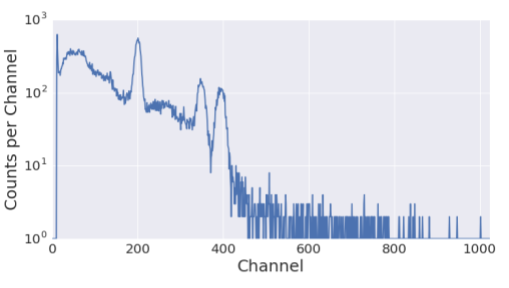
\includegraphics[width=0.7\linewidth]{images/CoCs_mix}
    \caption{Gamma-ray spectrum of a 0.288 $\mu$Ci $^{60}$Co source and a 0.890 $\mu$Ci $^{137}$Cs source. Each source-to-detector distance was adjusted so their respective count rate on the detector was equal.}
    \label{fig:top_five}
\end{figure}


\section{Dataset Construction}

In order to train an ANN, a training set and training key must be provided. The training set is a set of ANN input data and the training key is the correct ANN output for each input. Because creating a training set of real gamma-ray spectra is infeasible, the training set used in this work was simulated. The training set was created using a one-dimensional Monte Carlo radiation detector simulation program called GADRAS \cite{mitchell2014}. The simulation process began by simulating individual 1 mCi sources with no background. Each source was simulated at a distance of 30cm from a 2 inch by 2 inch Ortec 905-3 NaI spectrometer for 10 hours, ensuring each spectrum had low statistical noise. These single isotope sources were then sampled using the inverse transform sampling method \cite{Devroyne}. This allows the creation of arbitrary source combinations. The background isotopes were modeled using built-in GADRAS background sources for $^{40}$K, uranium and daughters in soil, and thorium and daughters in soil.

Because the calibration on NaI detectors shifts over time (due to voltage drift in the electronics and changes in crystal temperature), a method to change training spectra calibration was included. To mimic gain shift, the channels in each spectrum were linearly rebinned by some percent. The magnitude of each shift was uniformly chosen between a +/- 25\% gain drift. After rebinning, the resulting spectrum was reconstructed using third order spline interpolation with the new bin positions.


Using this method, many training sets can be created depending on different algorithm goals. The training set and isotope library can be modified for specific problems like unknown source interdiction and uranium enrichment calculations. Methods of creating ANNs for these problems will be described in later sections.

% The isotope library chosen for this demonstration was 29 gamma-ray producing isotopes from the ANSI N42.34-2006 standard, as well as $^{152}$Eu \cite{ANSI}. Based on lab observations using an Ortec 905-3 NaI spectrometer, the average background count rate was set at 85 counts per second (cps). Each spectrum in the training set had a maximum of 5 different non-background isotopes included in the spectrum. Each isotope had a count rate which was logarithmically distributed between 10 and 1000 cps. The exposure time was logarithmically distributed between 10 and 2000 seconds. Each isotope, excluding those in background, had an equal probability of being included in each spectrum. The counts from background were distributed uniformly between background thorium, background uranium, and background $^{40}$K.



\section{Training Details and Hyperparameter Optimization}

An optimization algorithm is needed to train the model. Optimization is necessary to choose good model parameters and hyperparameters. Model parameters are the weights connecting each layer in an ANN. Optimizing the model parameters is also known as training or learning. Hyperparameters are the variables that define the structure of the ANN (number of layers, nodes in each layer, non-linear function on each node) as well as the variables that control how the model learns (the learning rate, neuron dropout frequency, loss function). Finding appropriate hyperparameters requires trying different hyperparameter combinations and seeing which gives the lowest error on a validation dataset. This can be done using either a manual or automated search.

The Adam optimizer was chosen as the training algorithm for this work due to its incorporation of parts of other successful optimization algorithms and its reported superior performance over these algorithms \cite{Kingma2015}. Another benefit of the Adam optimizer is the introduction of only one additional hyperparameter, the learning rate. Other optimizers require tuning more than one additional hyperparameter. During training, the ANN minimized the average cross entropy,

\begin{equation} \label{eq:CrossEntropy}
E = -{\frac{1} N} \sum_{n=1}^N y_n \log(\hat{y}_n) +  (1-y_n) \log(1-\hat{y}_n),
\end{equation}

between each of the $N$ correct labels, $y_n$, and the $N$ network predictions, $\hat{y}_n$. This cost function was chosen because it is traditionally used with ANNs whose output is the softmax function. 

Raw data is typically preprocessed before being input to an ANN. For this work each spectrum was preprocessed by scaling the counts in each bin between [0,1]. Scaling the inputs improves numerical stability during training. 

Hyperparameters are often necessary to properly train an ANN. The following hyperparameters are considered in this study: the number of neurons in each layer, the number of layers used, initial learning rate for the training algorithm, the $L_2$ weight regularization strength, and neuron dropout rate. 

Adding $L_2$ weight regularization allows the magnitude of the weights to increase only when there is a comparable reduction in the unmodified error function,
%
\begin{equation} \label{eq:L2_Reg}
\tilde{E} = E + \sum_i \lambda w_i^2.
\end{equation}
%
In Equation \ref{eq:L2_Reg}, $w_i$ is the weight between each neuron in the ANN and $\lambda$ is the regularization strength hyperparameter. A larger $\lambda$ will force the ANN to prefer smaller weights connecting the neurons. This reduces the model's capacity, or its ability to represent complicated or intricate functions. This is similar to putting a limit on the magnitude of the coefficients in a high order polynomial when fitting data. If $\lambda$ is too small, the model will have too much capacity. This will create a model that is more likely to overfit. If $\lambda$ is too large, the ANN will preferentially minimize the $L_n$ error, failing to learn the desired task.

Another method to reduce model capacity is neuron dropout. Neuron dropout is the process of temporarily removing a neuron from the ANN architecture during training \cite{Srivastava2014}. The probability that a neuron is removed is called the neuron dropout rate, which is a hyperparameter. By applying dropout throughout training, the ANN's architecture changes every iteration. This makes neuron dropout a cost efficient way to average many different ANN architectures, improving performance.

% To reduce free parameters that might lead to overfitting, the number of neurons in each layer is typically smaller than the size of the input layer, in this case 1024. Another method of   Because  kept below 10$^{4}$.   


\section{Key Results}

Two key results are described in the following section. The first result demonstrates the ANN's ability to correctly identify isotopes in the ANSI N42-34-2006 library with an unknown calibration. This demonstration also demonstrates how well the ANN operates when spectroscopic features such as photopeaks are unclear. The second result demonstrates the ANN's ability to identify an isotope that is shielded by lead, distorting it's spectrum.  

\subsection{Single Isotope Identification}

The isotope library chosen for this demonstration was 29 gamma-ray producing isotopes from the ANSI N42.34-2006 standard, as well as $^{152}$Eu \cite{ANSI}. $^{152}$Eu has a large number of photopeaks over a wide range of energy. This makes it difficult to identify, especially with shielding. Because this isotope is available in our laboratory, where other isotopes with similar decay schemes are not, it is included in this study. Based on lab observations using an Ortec 905-3 NaI spectrometer, the average background count rate was set at 85 counts per second (cps). Each spectrum in the training set had a maximum of 5 different non-background isotopes included. Each isotope had a count rate which was logarithmically distributed between 10 and 1000 cps. Above this count rate, deadtime effects distort the spectrum. These effects are outside the scope of this study. The exposure time was logarithmically distributed between 10 and 2000 seconds. Each non-background isotope had an equal probability of being included in each spectrum. The counts from background were distributed uniformly between natural background thorium, background uranium, and background $^{40}$K. To mimic calibration shift, the channels in each spectrum were linearly rebinned. The magnitude of each shift was uniformly chosen between a +/- 25\% calibration drift. The 0\% gain shift setting corresponds to a detector with a maximum bin energy of 3 MeV. A calibration drift of +/- 25\% is an extreme case of incorrect calibration.

To demonstrate the performance of the algorithm on spectra with single isotopes where features were easily identifiable by eye versus spectra without obvious visible features, two simulated validation datasets were considered. Both datasets consisted of spectra with a single isotope simulated using the same process as the ANN training set with the rebinning randomly chosen between +/-20\%. The rebinning magnitude was reduced to avoid testing the ANN near the edge of it's training. A calibration drift of +/-20\% is still an extremely incorrect calibration. Two confusion matrices, shown in Figure \ref{fig:conf_matrix_60s} and \ref{fig:conf_matrix_10s}, were used to compare the performance of the ANN on both datasets. For all the results, the count contribution cutoff was arbitrarily set at 15\% of the largest count contribution calculated by the ANN.


For spectra in the first validation dataset, both the source and background contributed 85 counts per second with an integration time of 60 seconds. Each isotope in the training library was simulated one hundred times with this count distribution. Simulated $^{60}$Co spectra with the extreme calibration settings are shown in Figure \ref{fig:co60_diff_pmt_60s}.



\begin{figure}[H]
\centering
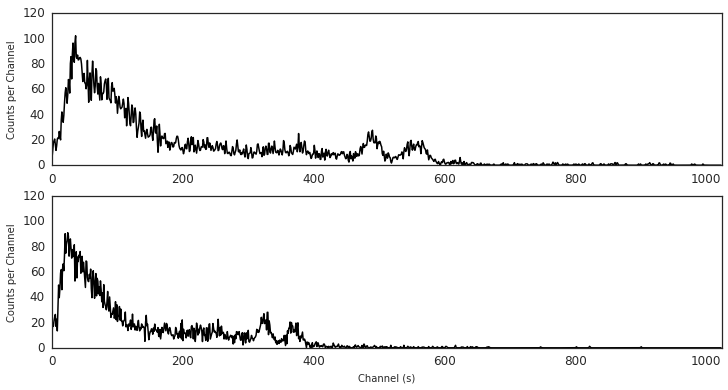
\includegraphics[width=0.75\linewidth]{images/Co60_both_60s}
\caption{Two simulated $^{60}$Co spectra. In each spectrum, the $^{60}$Co and background contribute 5100 counts to the spectrum. The bottom spectrum's gain was offset by -20\% while the top spectrum's gain was offset by +20\%.}
\label{fig:co60_diff_pmt_60s}
\end{figure}

The confusion matrix generated using an ANN is displayed in Figure \ref{fig:conf_matrix_60s}. In this confusion matrix, the largest count contributing isotope was used to identify the spectrum. The ANN exhibited a low false positive rate with this simulated dataset. False positives occurred mainly with sources that primarily emit only a few low-energy photons. This is especially notable when $^{99m}$Tc, which primarily emits a 141 keV gamma-ray, is misidentified as $^{57}$Co, which emits a 122 keV gamma-ray. A -13\% calibration shifted  $^{99m}$Tc spectrum looks almost identical to a $^{57}$Co spectrum without a calibration shift. Incorrect identification occurred due to the proximity of the photopeaks of these isotopes. Incorrect identification also occurred due to a lack of other prominent spectral features such as the Compton continuum for low-energy gamma-rays. This effect can also be seen in Figure \ref{fig:conf_matrix_60s} when $^{204}$Tl is misidentified as $^{201}$Tl. Both $^{204}$Tl and $^{201}$Tl primarily emit photons around 70 and 80 keV.




\begin{figure}[H]
\centering
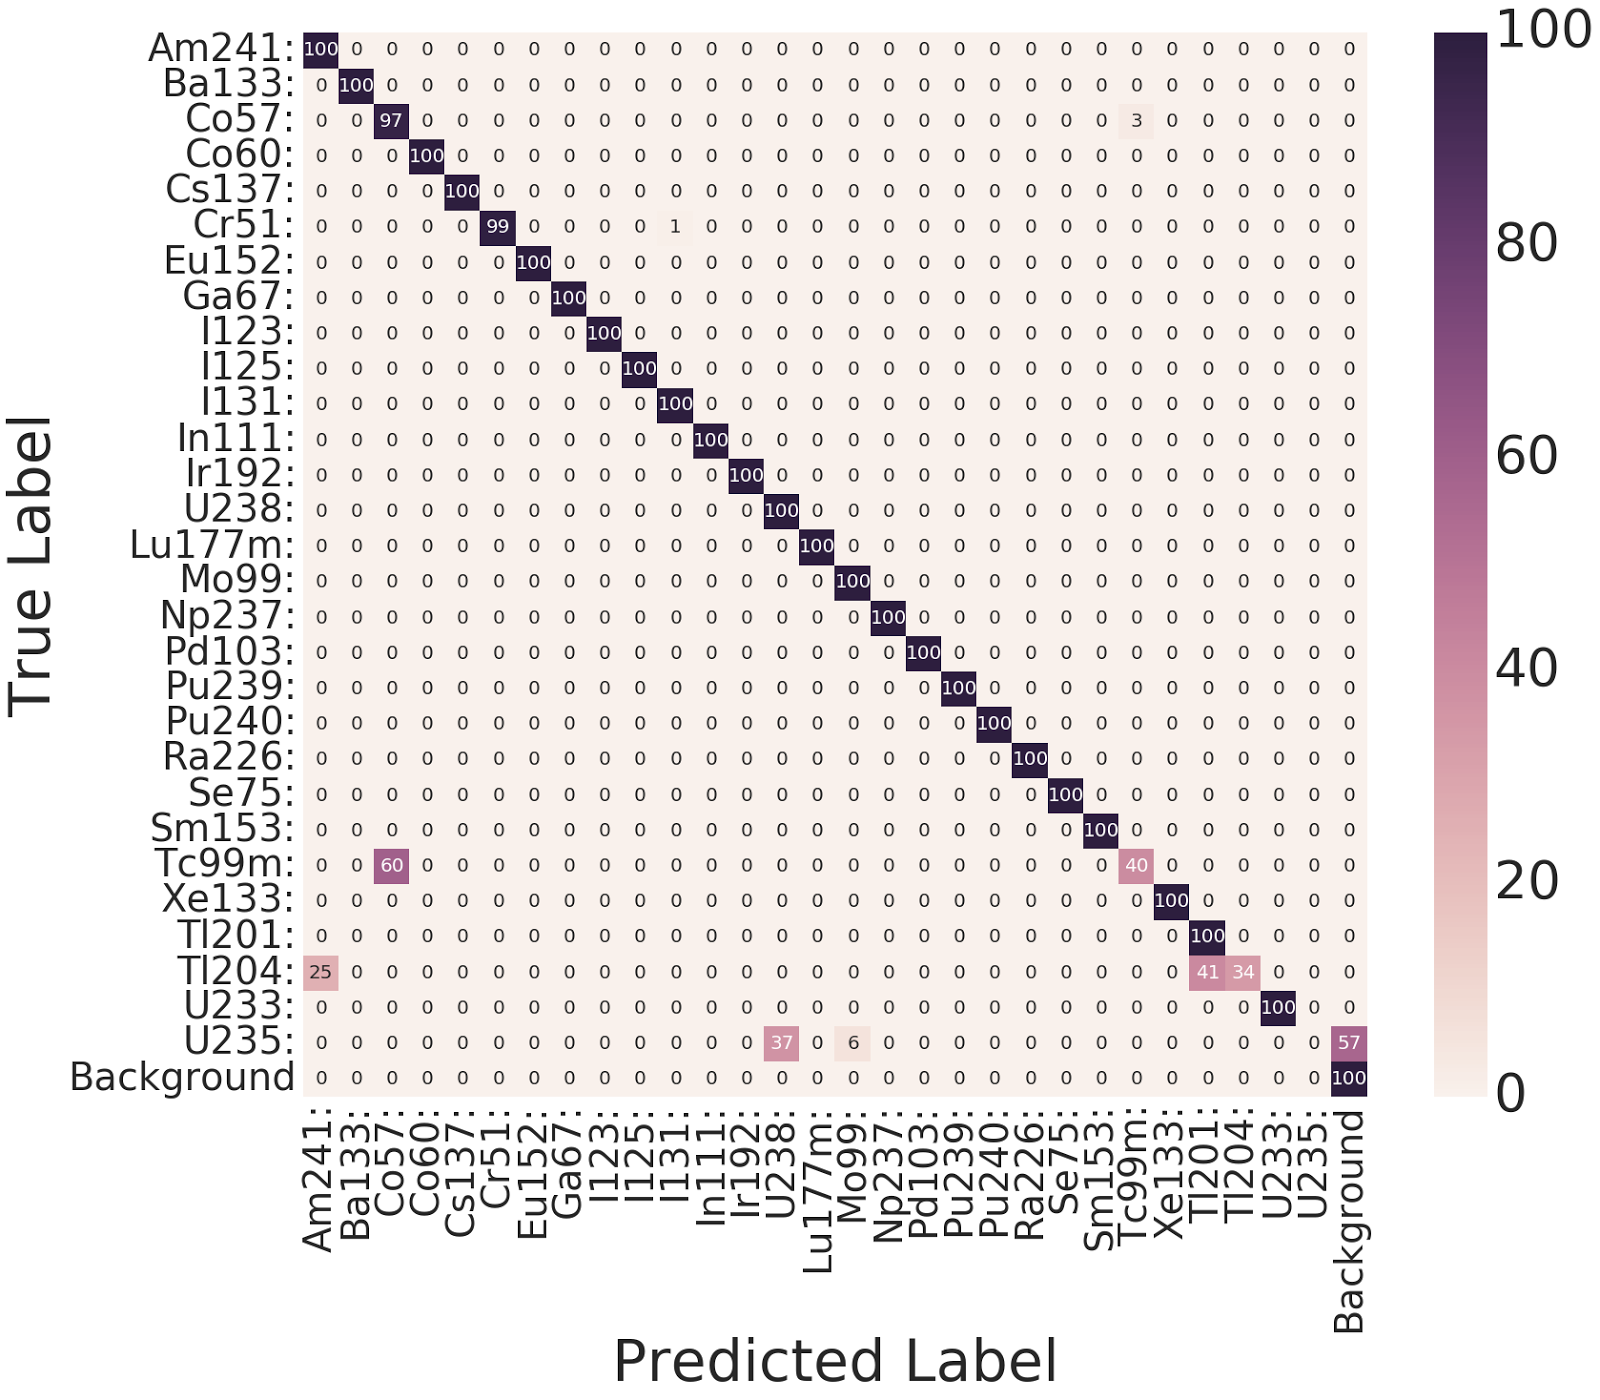
\includegraphics[width=0.9\linewidth]{images/conf_matrix_60s}
\caption{The confusion matrix for a single isotope dataset. Both the source and background contribute 5100 counts to the spectrum.}
\label{fig:conf_matrix_60s}
\end{figure}

In the second validation dataset, the source and background were simulated with an integration time of 10 seconds and the source count rate was reduced to half the strength of background. Example simulated $^{60}$Co spectra with the extreme calibration settings are shown in Figure \ref{fig:co60_diff_pmt_10s}. Note that compared to figure \ref{fig:co60_diff_pmt_60s}, the photopeaks of $^{60}$Co are more difficult to identify by eye. The lack of clear spectral features in these spectra may present extra difficulty to algorithms that rely solely on feature extraction methods. Also, the lack of prominent background peaks would make these spectra difficult to calibrate.

\begin{figure}[H]
\centering
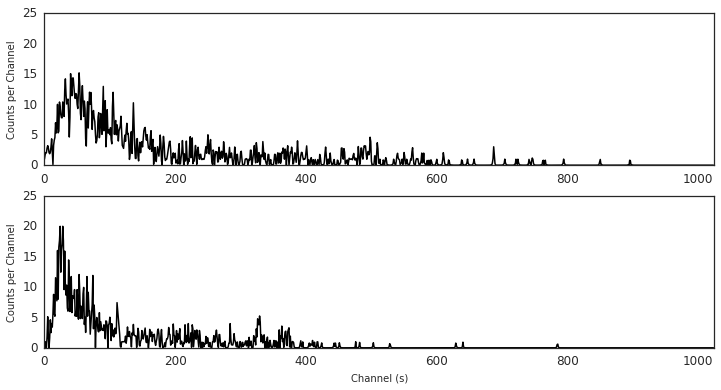
\includegraphics[width=0.75\linewidth]{images/Co60_both_10s}
\caption{Two simulated $^{60}$Co spectra. In each spectrum, the $^{60}$Co source contributes 425 counts and background contribute 850 counts. The bottom spectrum's gain is offset by -20\%, while the top spectrum's gain is offset by +20\%.}
\label{fig:co60_diff_pmt_10s}
\end{figure}

The confusion matrix for the second dataset is shown in Figure \ref{fig:conf_matrix_10s}. Note that the false positive rate increases, but often there was enough information in each spectrum to correctly identify the isotope. This implies that the ANN trained in this way can be effective in non-ideal measurement situations (low signal-to-noise spectrum, short measurement time, incorrectly calibrated detector).

\begin{figure}[H]
\centering
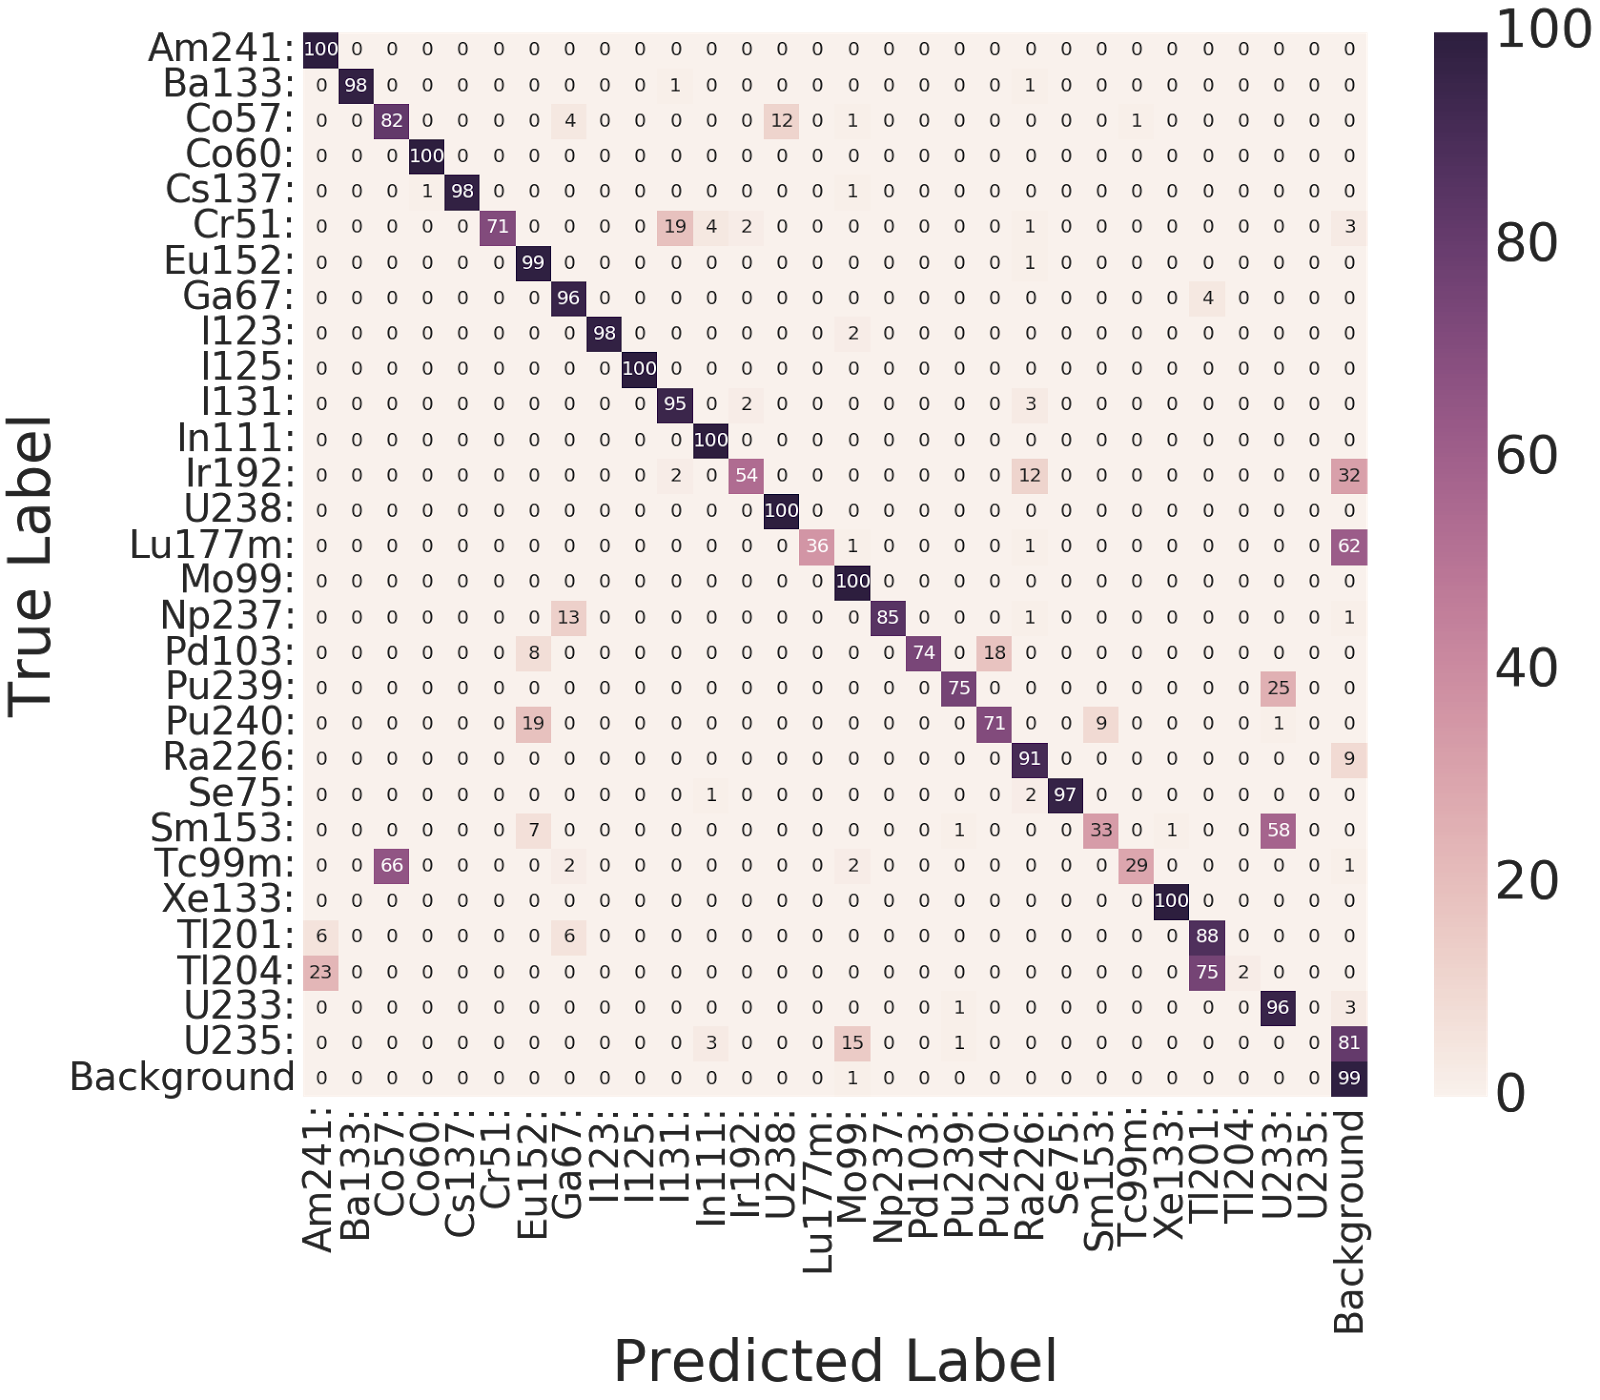
\includegraphics[width=0.9\linewidth]{images/conf_matrix_10s}
\caption{The confusion matrix for a single isotope dataset. In each case, the source contributes 425 counts and background contributes 850 counts to the spectrum.}
\label{fig:conf_matrix_10s}
\end{figure}

\subsection{Identifying Bare and Shielded $^{152}$Eu}

An ANN was trained to identify bare and shielded isotopes. The ANN used a training dataset composed of bare and shielded sources from the ANSI N42-34-2006 library.

The ANNs performance is displayed by identifying a bare and shielded $^{152}$Eu source. The $^{152}$Eu isotope emits gamma-rays in a large range of energies. Because lower-energy gamma-rays are attenuated more strongly than higher-energy gamma-rays, the shielded $^{152}$Eu spectrum, shown in Figure \ref{fig:Shielded_Eu152}, is significantly distorted compared to an unshielded $^{152}$Eu spectrum, shown in Figure \ref{fig:Bare_Eu152}. The effect of shielding can be seen by observing that the photopeaks below channel 100 observed in the bare source spectrum are not present in the shielded spectrum. In addition to distorting the spectrum, the shielding also reduced the number of counts in the spectrum, decreasing the signal-to-noise ratio. 

\begin{figure}[H]
\centering
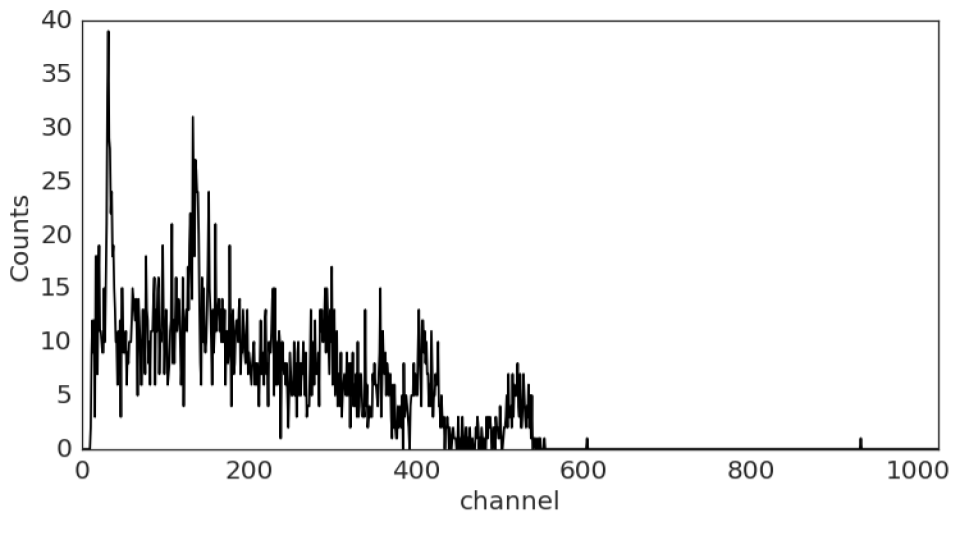
\includegraphics[width=0.75\linewidth]{images/Shielded_Eu152}
    \caption{Spectrum of a Eu152 10$\mu$Ci source shielded by 8mm of lead. The collection time for this was 10s.}
\label{fig:Shielded_Eu152}
\end{figure}

\begin{figure}[H]
\centering
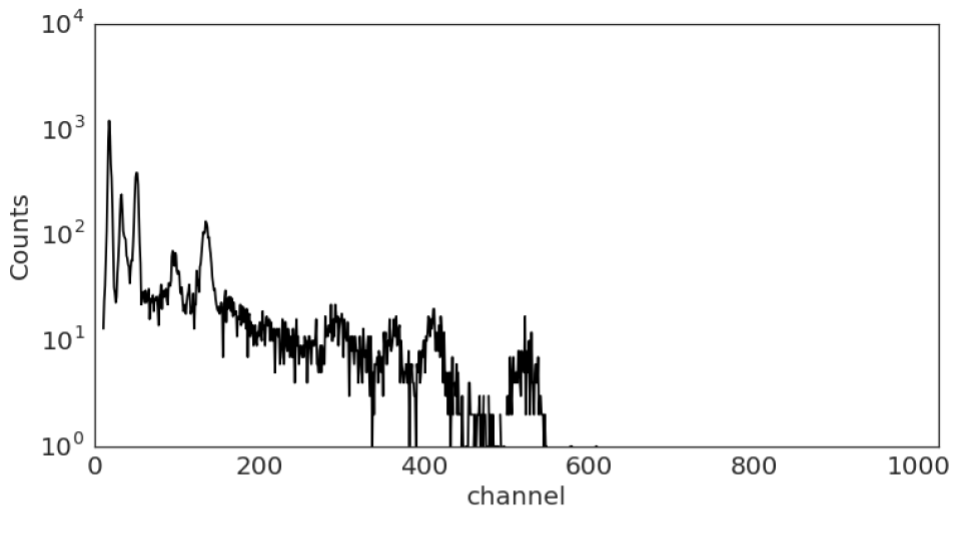
\includegraphics[width=0.75\linewidth]{images/Bare_Eu152}
\caption{Spectrum of a Eu152 10 $\mu$Ci source. The collection time for this was 10s.}
\label{fig:Bare_Eu152}
\end{figure}

Despite the distortion and lower signal-to-noise ratio in the shielded example, the ANN was able to differentiate a bare and shielded $^{152}$Eu source. The average ANN output from 5 bare 10 $\mu$Ci $^{152}$Eu spectra collected for 10 s is shown in Table \ref{table:Bare_Eu152_results}. Note that the ANN calculated that the vast majority of counts came from $^{152}$Eu and background. Table \ref{table:Shielded_Eu152_results} shows the average ANN output for 5 $^{152}$Eu spectra collected in the same manner as previous with the addition of an 8mm lead shield. While the top count contributor was shielded $^{152}$Eu, the ANN included a number of incorrect sources with high count contributions. The extra identifications are likely due to the low signal-to-noise ratio in the shielded spectrum.

\begin{table}[H]
\centering
\caption{Average ANN output from five spectra. Each spectrum was collected like the one in Figure \ref{fig:Bare_Eu152}. Only the top five isotopes are shown.}
\label{table:Bare_Eu152_results}
\begin{tabular}{|c|c|}
\hline
Isotope    & \begin{tabular}[c]{@{}c@{}}Count \\ Contribution\end{tabular} \\ \hline
$^{152}$Eu  & 0.496                                                         \\ \hline
Background $^{40}$K & 0.090                                                         \\ \hline
Background Uranium & 0.072                                                         \\ \hline
Background Thorium  & 0.056                                                         \\ \hline
$^{60}$Co  & 0.051                                                         \\ \hline
\end{tabular}
\end{table}




\begin{table}[H]
\centering
\caption{Average ANN output from five spectra. Each spectrum was collected like the one in Figure \ref{fig:Shielded_Eu152}. Only the top five isotopes are shown.}
\label{table:Shielded_Eu152_results}
\begin{tabular}{|c|c|}
\hline
Isotope    & \begin{tabular}[c]{@{}c@{}}Count \\ Contribution\end{tabular} \\ \hline
Shielded $^{152}$Eu  & 0.303                                                         \\ \hline
Shielded $^{238}$U & 0.234                                                         \\ \hline
$^{137}$Cs & 0.182                                                         \\ \hline
$^{131}$I  & 0.084                                                         \\ \hline
$^{60}$Co  & 0.074                                                         \\ \hline
\end{tabular}
\end{table}



\section{Chapter Conclusion}

This chapter illustrates a method to use an ANN to perform gamma-ray spectroscopy using the full gamma-ray spectrum. The chapter also discusses key results which while promising, can be improved. These improvements will be discussed in the next chapter.



%%%%%%%%%%%%%%%%%%%%%%%%%%%%%%%%%%%%%%%%%%%%%%%%%%%%%%%%%%%%%%%%%%%%%%%%%%%%%%%%%%%%%%%%%%%

% \section{Thesis and TNS Publication}

% The work I published has a lot of room for improvement. Some physics in the MCNP 6 model were neglected, like any radiation contribution from bremsstrahlung and environmental scatter. Also the background isotope spectra were very wrong. These were generated assuming a point source of radiation. Real background is distributed in the soil. Many scattering events in soil along with skyshine contribute to a spectrum that looks very different from a point source. %(cite MCNP background simulation paper). 

% There were parts of the published work that were good. The sampling method based on isotope templates is a good method to simulate lots of realistic gamma-ray spectra. One of the most difficult parts of ANN training is creating a good training set that represents reality. This method can be used to simulate most things, which is hugely useful. The results of the published work were also very promising. Despite the unrealistic physics model used in the simulation, the ANN correctly identified isotopes in a variety of simulated and real spectra. 

% Moving away from the MCNP model, we used GADRAS to create our template spectra. GADRAS has done all the physics heavy lifting for us, which is awesome. Also lets us simulate shielding, different scattering environments, detectors with different parameters(FWHM vs energy, nonlinear calibration, crystal dimensions), and entirely different detectors. We have demonstrated that an ANN trained with this data can accurately identify poor quality simulated spectra. Real spectra are still needed to verify these results.


% The current method begins by simulating a gamma-ray spectrum dataset for a given identification and quantification task. The ANN inputs are 1024 channels of a NaI spectrum and the output is percent count contributions from each isotope in the library used. The number of input channels can be easily changed to accommodate other detectors. 


% \section{Shielding Experiment Results}

% We're seeing some confusion in low-energy isotopes. Still need to validate results on real spectrum dataset. 

% \section{Uranium Enrichment Measurement Experiment}

% The ability for an ANN to perform isotope quantification for uranium enrichment measurements was investigated. This work also explored if dimension reduction techniques (PCA and autoencoders) improved ANN performance over using the full spectrum as ANN input. As seen in Figure \ref{fig:enrichment_error}, PCA and the autoencoder stopped learning before the full spectrum. This indicates that using the full spectrum as ANN input may be superior to using dimension reduction techniques for this problem. 


% Table \ref{fig:enrichment_MSE_table} also shows that using the full spectrum as ANN input is superior to dimension reduction techniques. This table also shows that the ANN is best at identifying $^{235}$U. The accuracy of $^{235}$U implies that ANN is not learning calibration drift well. The 186 keV peak from $^{235}$U has no overlap, even with gain drift, with the other isotopes in the training library. This allows the ANN to accurately identify it. Conversely, $^{231}$Th and $^{234}$Th emit similar low-energy gamma-rays. These become easily confused with gain drift. This implies that gain correction and isotope identification and quantification should be handled by a separate algorithms. Suggestions for improvements for this will be explained in later sections.


\chapter{Future Work and Proposed Experiments}

For the proposed work, a number of experiments that will explore applying ANNs to gamma-ray spectroscopy. An outline of this work can be seen in Figure \ref{fig:ANN_workflow}. Section \ref{ProposedDatasets} details two proposed gamma-ray spectra datasets to be simulated. Motivation is given to establish that these datasets represent important problems in gamma-ray spectroscopy. In addition to ANNs that use the full spectrum as input, ANNs that are trained to perform feature extraction will also be considered. Section \ref{Autoencoders} describes how autoencoders can be trained to extract key features from a gamma-ray spectrum. Section \ref{CrossValidation} describes how the random hyperparameter search will be performed using K-folds cross validation. Once an appropriate ANN is found, a method called bagging (bootstrap aggregating) will be used to construct an ensemble of ANNs. Bagging is described in Section \ref{Bagging}. Finally, the ANN performance on each dataset will be evaluated. Performance metrics are based on the ANN error in testing datasets, described in section \ref{ProposedDatasets}.%, and ANN confidence, described in \ref{ModelConfidence}. 




\begin{figure}[H]
\centering
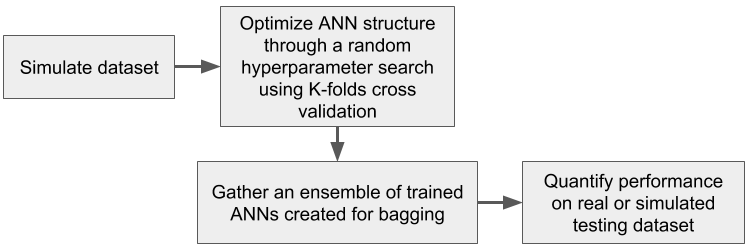
\includegraphics[width=0.8\linewidth]{images/ANN_workflow}
\caption{Workflow for the experiments proposed in this work.}
\label{fig:ANN_workflow}
\end{figure}



\section{Proposed Datasets} \label{ProposedDatasets}

The proposed datasets represent important problems in automated gamma-ray spectroscopy. These include unknown source interdiction, uranium enrichment calculations, and isotope mixture analysis. 

\subsection{Unknown Source Interdiction} \label{UnknownSourceInterdiction}

One important problem in automated gamma-ray spectroscopy is giving untrained operators the ability to identify an unknown source. Performance requirements for this task are outlined in the ANSI N42-34-2006 standard. For this reason, this standard will guide the requirements in this section. Issues addressed by the ANSI standard include unknown shielding, unknown detector calibration, and unknown source combination. Methods to address these issues by using an ANN are described below. A way to validate the results is also described. 

Typically, a source will be shielded, producing a weaker signals and distorting the spectrum. To address this, the training dataset will be sampled from a library of bare and shielded spectra. Because different materials have different shielding properties, a variety of shielding materials and thicknesses will be included in the library. The materials included will be common shields, including aluminum, iron, and lead. The thicknesses will correspond to the amount needed to attenuate 662 keV gamma-rays by 20\%, 40\%, 60\%, and 80\%. These thicknesses can be seen in Table \ref{table:Shielding_to_include}.

\begin{table}[H]
\centering
\caption{Different amounts of aluminum, iron, and lead shield included in the training library.}
\label{table:Shielding_to_include}
\begin{tabular}{c|c|c|c|c|}
\cline{2-5}
                               & 20\% & 40\% & 60\% & 80\% \\ \hline
\multicolumn{1}{|c|}{Aluminum} & 1.0 cm  & 2.3 cm  & 4.1 cm & 7.2 cm \\ \hline
\multicolumn{1}{|c|}{Iron}     & 0.38 cm  & 0.87 cm  & 1.6 cm & 2.8 cm  \\ \hline
\multicolumn{1}{|c|}{Lead}     & 0.18 cm  & 0.42 cm  & 0.76 cm  & 1.3 cm \\ \hline
\end{tabular}
\end{table}

% In addition, medical isotopes should be simulated/tested using polyethylene as a shield to simulate the human body.

Because untrained operators would be using these algorithms, the detector calibration cannot be trusted. To address this, in each training batch the channels in each spectrum will be rebinned. This rebinning will be based on the calibration of real detectors in our lab have at different photomultiplier tube (PMT) voltages. Typically these will be set at 750 V, corresponding to an energy range between 40 keV - 3000 keV. This energy range includes the gamma-rays required to identify isotopes in the ANSI library. The range of incorrect calibration will include 700 V - 800 V.

The ANSI standard also includes the ability to identify isotope mixtures in their requirements. The ANSI standard is primarily interested in combinations of special nuclear material (weapons grade plutonium (WGPu), high enriched uranium (HEU)) with medical isotopes (e.g., $^{99m}$Tc, $^{201}$Tl, or $^{67}$Ga). To address this, random mixtures of one, two, and three isotopes will be included in the training dataset.

To fit the source interdiction scenario, count rate and source measurement time for spectra in the simulated training set will be kept within a range. The count rate on the detector will range from 10 counts per second (cps) to 10$^{4}$ cps. Below 10 cps the signal-to-background ratio will be too low for an identification. Above 10$^{4}$ cps deadtime effects will distort the spectrum. Sources above this count rate are easy to detect and would receive additional scrutiny. Source measurement times will range from 10 s - 1 hr. This is a typical range of measurements for source interdiction. 

The performance of the ANN on this dataset will be reported in several ways. The ability to detect isotopes behind shielding will be tested by observing how the ANN identifies various laboratory isotopes behind shielding. Sources for this will include $^{60}$Co, $^{137}$Cs, $^{152}$Eu, and $^{133}$Ba. These sources are chosen because they are available in our laboratory, and they represent isotopes with simple gamma-ray spectra ($^{60}$Co and $^{137}$Cs have two identifiable photopeaks) and more complicated spectra ($^{152}$Eu and $^{133}$Ba have multiple photopeaks over a wide range of energies). In addition to laboratory sources, real and simulated spectra of shielded HEU and WGPu will be included in this analysis. The mean ANN outputs and their variances will be presented for a number of spectra. 

The ANNs ability to identify spectra with various calibrations will also use $^{60}$Co, $^{137}$Cs, $^{152}$Eu, and $^{133}$Ba. Spectra of individual sources will be measured using various calibrations. The calibration will be changed by changing the PMT voltage from 700 V to 800 V in 10 V steps. The mean ANN outputs and variances will be presented for a number of spectra. 

The ANNs ability to identify mixtures of less than three isotopes will be addressed. Mixtures of $^{60}$Co, $^{137}$Cs, $^{152}$Eu, and $^{133}$Ba will be recorded. The mean ANN outputs and their variances will be reported. In addition to these, mixtures in required by the ANSI standard, 

\begin{itemize}
  \item $^{137}$Cs + depleted uranium (DU)
  \item $^{99m}$Tc + HEU
  \item $^{201}$Tl + HEU
  \item $^{67}$Ga + HEU
  \item $^{131}$I + WGPu
  \item Naturally occurring radioactive material (NORM) + HEU
  \item NORM + WGPu
\end{itemize}

will be simulated and their mean ANN output and variance will be reported. 



% using a ROC curve and confusion matrix for a simulated spectra dataset. The dataset will be based on the dataset used to train the ANN. This will give information on how well the ANN can operate on the dataset it was trained to identify. 

\subsection{Uranium Enrichment Calculations}

Measuring the enrichment of uranium is important for treaty verification purposes. These measurements are performed in uranium enrichment facilities and to verify warhead disarmament. Due to treaty conditions limiting the amount of sensitive information released to inspectors, information barriers are required. Information barriers can include removing regions in gamma-ray spectra or giving no information about shielding between the source and detector. 

ANNs are a good candidate as an information barrier for three reasons. First, their output can be constrained, only outputting the enrichment given a gamma-ray spectrum. Restricting the output ensures potentially sensitive details of the sample are not known. Second, ANNs can be trained to use spectra with unknown background radiation and calibration drift. Because the inspector will have a time constraint, it is assumed a separate background spectrum will not be taken. By varying the background in the training set, ANNs can be taught to operate with different background radiation. The other unknown, possible calibration drift, is typically corrected manually. Because the inspector will not have access to the spectrum, manual calibration adjustments cannot be performed. It has been shown that ANNs can be taught to identify isotopes in detectors with different calibration.  \iffalse Finally, the ANNs confidence in its predictions can be calculated. Low confidence predictions could indicate a hoax object has been measured. \fi A few technical hurdles need to be addressed when constructing an ANN to perform uranium enrichment. These hurdles and methods to address them are described below.

Because uranium emits relatively low energy gamma-rays, it's spectrum is especially susceptible to corruption by shielding. To address this, a shielding library will be included in the dataset simulation. This will be constructed using the same method described in section \ref{UnknownSourceInterdiction} using the material thicknesses shown in Table \ref{table:Shielding_to_include}.

Treaty verification inspectors typically have under an hour to collect data for an enrichment measurement. For this reason source measurement times will range from 5 mins to 1 hr. Collection times shorter than 5 mins may produce ANNs with \iffalse low confidence and \fi high variance outputs. To demonstrate the ANNs performance versus collection time, a graph of the measurement time versus ANN accuracy \iffalse and confidence \fi  on a simulated verification dataset will be included. It is expected that collecting times less than 10 mins will result in an ANN accuracy too low to be of practical use. For reference, analytically chemical techniques can measure uranium enrichment to 0.1-0.2\% accuracy \cite{Pandas_Ch7_1991}. Comparing the areas of photopeaks in HPGe spectra, an accuracy of about 1\% is possible \cite{Pandas_Ch7_1991}. Also due to the time constraint, it is assumed that background data cannot be collected. To address this, each training sample will include a random combination of background isotopes. The background count rate will range from 10-120 cps.


Because trained inspectors are performing these measurements, large calibration drifts are not included in the training data. Small calibration drifts of less than 5\% will be included to account for temperature changes and electronic drift.

The isotope library necessary for uranium enrichment consists of only six isotopes: $^{235}$U, $^{238}$U, $^{234}$U, $^{234}$Th, $^{231}$Th, and $^{234m}$Pa. These are the main gamma-ray producing isotopes in a sample of uranium. The training set will be simulated using combinations of all of these isotopes in pseudo-random combinations. Random sampling does not guarantee the training space is evenly sampled and often produces clusters. The presence of clusters in the training set may lead the ANN to learn a bias for certain combinations of isotopes. A way to reduce the chances of clusters and more uniformly sample the input space is using Latin hypercube sampling (LHS). LHS partitions each dimension of a space into N equal parts. The space is then sampled using N points, ensuring that there is only one point along each partition in each dimension. An example of this sampling method for a two-dimension space is shown in Figure \ref{fig:LHS_example}.

\begin{figure}[H]
\centering
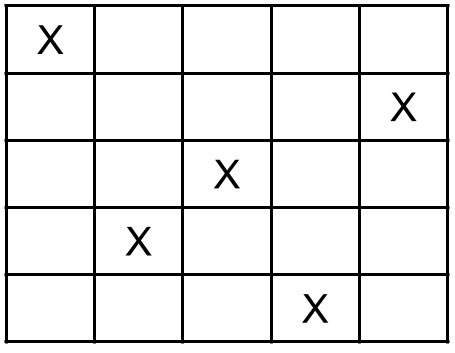
\includegraphics[width=0.4\linewidth]{images/LHS_example}
\caption{An example of LHS sampling. Seen here is a square sampled using five points.}
\label{fig:LHS_example}
\end{figure}

To quantify how much LHS helps identification, datasets will be constructed using random sampling and LHS. The number of samples in each dataset will be 1k, 5k, 10k, 50k, 100k. ANNs will be trained using these datasets and their  performance on a simulated validation dataset will then be measured and compared. It is expected that at a certain number of samples the ANN performance will reach an asymptote. It is also expected that the LHS datasets will reach a higher-accuracy asymptote quicker than the randomly sampled datasets. 


To test the ability for ANNs to measure uranium enrichment, depleted, low-enriched, medium-enriched, and high-enriched uranium spectra will be simulated. For each enrichment level, 100 spectra will be simulated using collection times of 5, 10, 60, 300, 600, 1800, and 3600 s. Each of these spectra will contain an unknown background and calibration similar to the training set. Separate validation sets will be constructed for a small amount of shielding (0.1 cm of lead) and a large amount of shielding (1 cm of lead). 

% http://citeseerx.ist.psu.edu/viewdoc/download?doi=10.1.1.541.4867&rep=rep1&type=pdf


% \subsection{Post-Detonation Nuclear Forensic Debris Analysis}


\iffalse
\subsection{Isotope Mixture Analysis}

% Immediately after a nuclear detonation, first responders may be collecting a large number of gamma-ray spectra using handheld low-resolution detectors. These detectors may have an unknown or poor calibration and each spectrum may be measured for a short amount of time. Despite these drawbacks, the data is still valuable because it can potentially be used to determine isotopics of the debris generated by the explosion \cite{Moody}. Due to the complicated gamma-ray spectrum produced by a large number of radioactive fission products, many photopeaks and spectral features will overlap in a spectrum. This feature overlap increases the difficulty of and slows photopeak analysis, especially for low-resolution spectrometers. 

Identifying mixtures of isotopes is important for two reasons. The first is that isotope mixtures may confuse identification algorithms by occluding important.

Mixture identification is particularly difficult for NaI detectors 

A real dataset of real spectra are needed to confirm the models performance. Mixtures of laboratory isotopes can be made. Mixtures will vary by signal-to-background ratio by varying source-to-detector distance and integration time. Isotopes available are: $^{60}$Co, $^{137}$Cs, $^{133}$Ba, $^{152}$Eu, $^{22}$Na and others. % Details to come....



One important question is how many combinations to include in the training set. To address this, datasets will be created including single isotope spectra, a max of 5 isotope spectra, and a max of 10 isotope spectra. ANNs will be trained with increasing number of examples (1k, 5k, 10k, 50k, 100k). The performance of these ANNs will be compared by observing how the 

\fi

\subsection{Additional Simulated Detector Models}

Simulating additional NaI detectors using GADRAS may help the ANN generalize to different detectors. To begin this process, two 2-inch by 2-inch NaI detectors will be modeled using GADRAS and their properties will be changed. These changes will include changing the calibration and changing the shape of the photopeaks. The calibration changes will be based on laboratory NaI detectors. The shape of photopeaks will be changed based on laboratory NaI detectors' full-width-at-half-max (FWHM). Ten different models will be included. 

Initial hyperparameter searches will be based on datasets simulated using a single detector. After an optimal ANN structure is found using the hyperparameter search, two new training datasets will be constructed with additional detector models. The two datasets will be constructed from five models and ten models. Two ANNs will be trained using both datasets. The performance of the ANNs on a dataset constructed using five new detector models will be reported. It is expected that the ANN trained using more detector models will have a higher accuracy on the new testing dataset. 


\section{Autoencoders} \label{Autoencoders}

% While autoencoders were touched on in the uranium enrichment work, they have not been explored thoroughly. There is some evidence that the autoencoder was overtrained to the A special case of denoising autoencoders will be explored for the ANSI dataset. 

An autoencoder is an ANN whose goal is to learn a representation of the input. This is accomplished by simultaneously training an encoding ANN and a decoding ANN. An example of this can be seen in Figure \ref{fig:Autoencoder_structure}. As seen in this figure, the encoding ANN reduces an $n-$dimension input signal, $X$, to a $m-$dimension signal, $z$, where $m < n$. The decoding ANN takes the encoded signal, $z$, and outputs a reproduction of the input signal, $X'$.

Without an autoencoder, a single ANN has to learn multiple tasks to identify isotopes. An ANN would have to simultaneously identify the detector calibration, background signal, and possible source signal. By training an autoencoder to reconstruct a background-subtracted and correctly calibrated spectrum, the task of isotope identification is simplified for the ANN. This may result in more accurate identifications. To test this, for each dataset a single autoencoder and three ANNs will be trained. The first will be trained without an autoencoder. The second will be trained using the encoder as input. The third will be trained using the full autoencoder as input. A random hyperparameter search will be used to find an appropriately structured autoencoder. The testing and validation error for these ANNs will be compared for each respective dataset.

% is local spatial structure too much jargon? 
In addition to using fully connected autoencoders, a 1-D convolutional autoencoder will also be explored. Fully connected ANNs do not assume the input has local spatial structure, while convolution ANNs do. Because gamma-ray spectra have local spatial structure in the form of photopeaks and Compton continua, it may be better to use a convolutional ANN over a fully connected ANN. To test this, the experiment described above will be repeated using a 1-D convolutional autoencoder.

% Or I might just use the 1D convolutional autoencoder because it makes more sense

\begin{figure}[H]
\centering
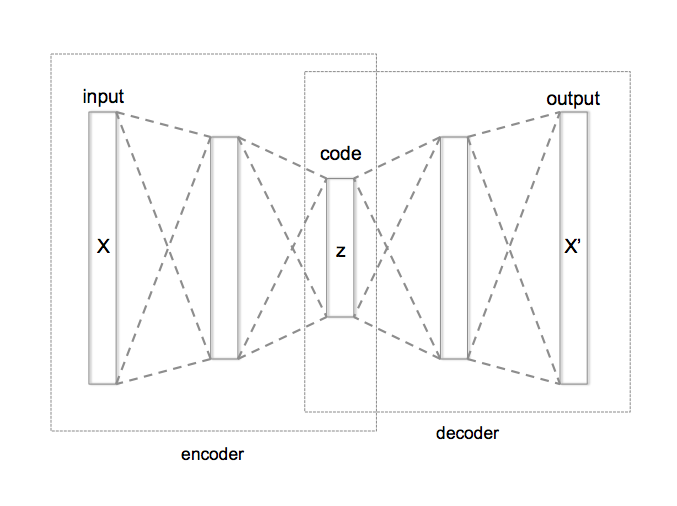
\includegraphics[width=0.8\linewidth]{images/Autoencoder_structure}
\caption{An example of an autoencoder \cite{wiki:AutoencoderStructure}.}
\label{fig:Autoencoder_structure}
\end{figure}


% Fully connected ANNs do not assume there is local spatial structure in a signal, so the fully connected ANN would need to learn that there is local structure. Convolutional ANNs assume there is local structure, and the extent of this structure can be changed by changing the length of the convolutional ANNs filters.

% Once the autoencoder is trained, the hidden layer and output layer (representing the reconstructed spectrum) will be used to train a separate ANN for isotope identification and quantification. The performance of these ANNs will be compared.




\section{K-folds Cross Validation} \label{CrossValidation}

% section is good.
K-folds cross validation will be included in the hyperparameter search for each dataset. Cross validation is the general method of determining how well a model will generalize to novel data. K-folds cross validation does this by splitting the available data into $k$ subsets. From these, $k-$1 subsets are used to train the ANN and the remaining subset is used as the validation dataset. Typical values for $k$ are either 5 or 10. This process is repeated, using each subset once as the validation dataset. This process is illustrated in Figure \ref{fig:kfolds_example} for 5-folds cross validation. 

For each different hyperparameter combination, a new set of cross validation ANNs will be trained. The average of the final validation dataset errors will be used to pick the optimal ANN. Performing cross validation will more accurately demonstrate how well a given set of hyperparameters will generalize to new data. For each dataset the error and hyperparameter structure will be compared for ANNs trained with no cross validation, 5-folds cross validation, and 10-folds cross validation.



\begin{figure}[H]
\centering
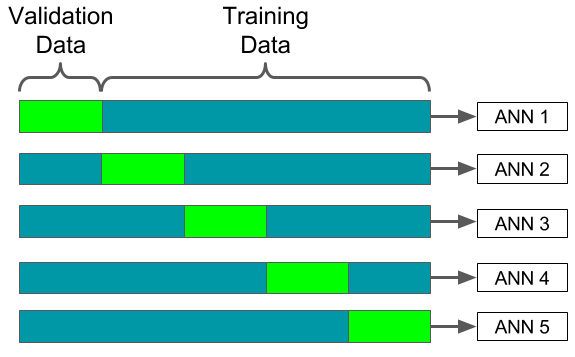
\includegraphics[width=0.6\linewidth]{images/kfolds_example}
\caption{An example of 5-folds cross validation. In each fold, the same dataset is partitioned into training data, in blue, and validation data, in green. Each training dataset is used to train a separate ANN. Each ANNs respective validation dataset is used to stop the ANNs training.}
\label{fig:kfolds_example}
\end{figure}




\section{Bagging} \label{Bagging}
% section is good.
Each time the ANN trains, it produces slightly different identification results and performance. Bagging, or the process of averaging the outputs of many ANNs, can reduce the variance in the output \cite{Breiman1996}. In addition to this, bagging more accurately displays the true performance of a given ANN structure.

Analyzing the performance of bagging begins once the ANN structure is found from the random hyperparameter search. Using this structure, ten models will be trained. Each model will use the entire training dataset, ending training at the average iteration used for the cross validation step. The accuracy and variance in the output as more models are averaged will be reported. The accuracy and variance are expected to plateau with enough models being averaged. If the accuracy or variance do not plateau after ten models, additional will be created until the effect is observed.

% future future work can explore boosting with these ANNs or weak learners. Could be very interesting. Also, weak learning models can be made tiny, possibly improving run-time without sacrificing (or even improving on) performance. 

\iffalse
\section{Model Confidence Using the Dropout Uncertainty Method} \label{ModelConfidence}

The dropout method used to regularize the ANN can be exploited to get a confidence measure on a given spectrum \cite{Yarin2016}. Once the ANN is trained, an input is given to the model and the output is recorded. Dropout is then used on the model using the same dropout probability that was used to train the model. The same input is then passed through the ANN and the answer recorded. The dropped neurons are restored and the process of dropout and recording the resulting output is repeated. Using this process, 

\begin{equation} \label{eq:update1}
E (y^{*}) \approx \frac{1}{T} \sum^{T}_{t=1} \hat{y^{*}_t} (x^{*})
\end{equation}

gives the average output given some input $x^{*}$, where $\hat{y}$ is the model output and T is the number of times dropout was performed. The variance of the outputs is given by 


\begin{equation} \label{eq:update1}
Var (y^{*}) \approx \tau^{-1} \boldsymbol{I}_D + \frac{1}{T} \sum^{T}_{t=1} \hat{y^{*}_t} (x^{*})^{T} \hat{y^{*}_t}(x^{*}) - E(y^{*})^{T}E(y^{*})
\end{equation}

where D is the length of the output vector and $\tau$ is defined by 

\begin{equation} \label{eq:update1}
\tau = \frac{l^2 p }{2 N \lambda}
\end{equation}

where $l$ is the prior length-scale, p is the probability of a neuron not being dropped, N is the length of the input vector, and $\lambda$ is the learning rate of the ANN. The prior length-scale, $l$ is a user defined parameter. A small valued $l$ corresponds to high frequency data and a larger valued $l$ corresponds to low frequency data. 


A few results are predicted using the ANN confidence. It is expected that high signal-to-background measurements and isotope mixtures of a few components will have a high model confidence. It is expected that low signal-to-background measurements and mixtures of many components will have a low model confidence. Additionally, the model confidence with an isotope not included in the training set should be very low. This confidence measure may be used to reduce the false alarm rate when performing isotope identification. 
 \fi
% \section{New Training Stopping Condition}

%%% Might still use this in the analysis. Might check that it changes anything for a few cases. Adds another degree of freedom in what I'm analyzing. Exponentiates number of things I need to test, without clear reason for benefit. 

% ANNs need a condition to end training. This condition is typically when a certain allowable error in a validation dataset is reached or when the training error does not appreciably decrease over time. Previously in this work, the stopping condition has been based on the cost function the ANN is trying to decrease, the cross entropy. It may be better to stop training when a more useful metric. An example of this metric is when the maximum error in the training set reaches a certain threshold. Another metric is to stop training when the ANNs mean squared error for a validation set stops decreasing.

\section{Chapter Conclusion}

The proposed datasets and ANN methods will directly serve key needs in domestic nuclear security and verification technology. Adding shielded spectra to the unknown source interdiction dataset will fulfill the requirements for shielded isotope identification in the ANSI N42-34-2006 standard. In addition to this dataset, the uranium enrichment dataset and ANN may provide an enrichment calculation algorithm that incorporates information barriers, can operate in areas with unknown background, and can operate without manual calibration adjustments. Finally, a dataset improvement in the form of incorporating additional detector models into the training dataset may increase the overall generalization performance of the ANN. 

The ANN methods explored in this section will more accurately display the performance of the ANN for each task. K-folds cross validation will make the hyperparameter search process more robust. Bagging will give a method to decrease the variance of the model, improving identification and more accurately displaying ANN performance. Finally, by taking advantage of the local structure in gamma-ray spectra, autoencoders will be explored for each tasks. 



\chapter{Conclusion}

Because of their flexibility and their ability to train using simulated data, ANNs are well suited to solving different problems in gamma-ray spectroscopy. Because ANNs incorporate fuzzy logic, they mimic the intuition a trained spectroscopist uses when identifying spectra. This is in contrast to other identification algorithms that use rigid rules which may struggle to identify spectra that are poorly calibrated, have insufficient counts to form obvious features, or are in an unknown background. 

To better understand what scenarios the ANN can operate in, two datasets will be investigated. The goal of the first dataset is to perform source interdiction using the ANSI N42-34-2006 library. The second dataset corresponds to performing uranium enrichment calculations for treaty verification purposes. %The final dataset will correspond to a source mixture problem using the ANSI N42-34-2006 library. This will be used as a surrogate for post-detonation nuclear forensics debris analysis. 

In addition to these datasets, a number of ANN experiments are suggested to improve on past work. The first improvement is adding additional detector models to the training set. The additional models should increase the generalization performance of the ANN. The second improvement will focus on how autoencoders can improve performance by keeping the calibration correction and background subtraction step separate from an ANN used for identification. This will include investigating the use of a 1-D convolution ANN as an autoencoder. To more accurately display the performance of a given ANN structure, k-folds cross validation will be added to the hyperparameter search for each dataset. After training, bagging  \iffalse and  model  confidence \fi will be added to the model. Bagging lowers the variance on the outputs of a given ANN structure and more accurately displays its performance.









\bibliographystyle{IEEEtran} % Dunno what format they want this!!! -MK 9/19/16
\bibliography{refs}

\end{document}

